\documentclass[english, 11 pt, class=article, crop=false]{standalone}
%\documentclass[english, 11 pt]{report}
\usepackage[T1]{fontenc}
\usepackage[utf8]{luainputenc}
\usepackage{babel}
\usepackage[hidelinks, bookmarks]{hyperref}
\usepackage{geometry}
\geometry{verbose,tmargin=1cm,bmargin=3cm,lmargin=4cm,rmargin=4cm,headheight=3cm,headsep=1cm,footskip=1cm}
\setlength{\parindent}{0bp}
\usepackage{amsmath}
\usepackage{amssymb}
\usepackage{esint}
\usepackage{import}
\usepackage[subpreambles=false]{standalone}
%\makeatletter
\addto\captionsenglish{\renewcommand{\chaptername}{Kapittel}}
\makeatother
\usepackage{tocloft}
\addto\captionsenglish{\renewcommand{\contentsname}{Innhold}}
\usepackage{graphicx}
\usepackage{placeins}
\raggedbottom
\usepackage{calc}
\usepackage{cancel}
\makeatletter
\usepackage{color}
\definecolor{shadecolor}{rgb}{0.105469, 0.613281, 1}
\usepackage{framed}
\usepackage{wrapfig}
\usepackage{bm}
\usepackage{ntheorem}

\usepackage{ragged2e}
\RaggedRight
\raggedbottom
\frenchspacing

\newcounter{lign}[section]
\newenvironment{lign}[1][]{\Large \refstepcounter{lign} \large
	\textbf{\thelign #1} \rmfamily}{\par\medskip}
\numberwithin{lign}{section}
\numberwithin{equation}{section}
\usepackage{xcolor}
\usepackage{icomma}
\usepackage{mathtools}
\usepackage{lmodern} % load a font with all the characters
\usepackage{xr-hyper}
\makeatother
\usepackage[many]{tcolorbox}

%\setlength{\parskip}{\medskipamount}
\newcommand{\parskiplength}{11pt}
%\setlength{\parskip}{0 pt}
\newcommand\eks[2][]{\begin{tcolorbox}[enhanced jigsaw,boxrule=0.3 mm, arc=0mm,breakable,colback=green!30] {\large \textbf{Eksempel #1} \vspace{\parskiplength}\\} #2 \vspace{1pt} \end{tcolorbox}\vspace{1pt}}

\newcommand\fref[2][]{\hyperref[#2]{\textsl{Figur \ref*{#2}#1}}}
\newcommand{\hr}[2]{\hyperref[#2]{\color{blue}\textsl{#1}}}

\newcommand\rgg[2][]{\begin{tcolorbox}[boxrule=0.3 mm, arc=0mm,colback=orange!55] #2 \vspace{1pt} \end{tcolorbox}\vspace{-2pt}}
\newcommand\alg[1]{\begin{align*} #1 \end{align*}}
\newcommand\algv[1]{\vspace{-11 pt} \begin{align*} #1 \end{align*}}
\newcommand\vs{\vspace{-11 pt}}
\newcommand\g[1]{\begin{center} {\tt #1}  \end{center}}
\newcommand\gv[1]{\begin{center} \vspace{-22 pt} {\tt #1} \vspace{-11 pt} \end{center}}
%\addto\captionsenglish{\renewcommand{\contentsname}{Løsningsforslag tentamen R2 H2015}}

% Farger
\colorlet{shadecolor}{blue!30} 

% Figur
\usepackage{float}
\usepackage{subfig}
\captionsetup[subfigure]{labelformat=empty}
\usepackage{esvect}

\newcommand\sv{\textbf{Svar:} \vspace{5 pt} \\}

%Tableofconents
\renewcommand{\cfttoctitlefont}{\Large\bfseries}
\setlength{\cftsubsecindent}{2 cm}
\newcommand\tocskip{6 pt}
\setlength{\cftaftertoctitleskip}{30 pt}
\setlength{\cftbeforesecskip}{\tocskip}
%\setlength{\cftbeforesubsecskip}{\tocskip}

%Footnote:
\usepackage[bottom, hang, flushmargin]{footmisc}
\usepackage{perpage} 
\MakePerPage{footnote}
\addtolength{\footnotesep}{2mm}
\renewcommand{\thefootnote}{\arabic{footnote}}
\renewcommand\footnoterule{\rule{\linewidth}{0.4pt}}

%asin, atan, acos
\DeclareMathOperator{\atan}{atan}
\DeclareMathOperator{\acos}{acos}
\DeclareMathOperator{\asin}{asin}

%Tabell
\addto\captionsenglish{\renewcommand{\tablename}{Figur}}

% Figur
\usepackage[font=footnotesize,labelfont=sl]{caption}
\addto\captionsenglish{\renewcommand{\figurename}{Figur}}

% Figurer
\newcommand\scr[1]{/home/sindre/R/scr/#1}
\newcommand\asym[1]{/home/sindre/R/asymptote/#1}

%Toc for seksjoner
\newcommand\tsec[1]{\phantomsection\addcontentsline{toc}{section}{#1}
	\section*{#1}}
%\newcommand\tssec[1]{\subsection*{#1}\addcontentsline{toc}{subsection}{#1}}
\newcommand\tssec[1]{\subsection*{#1}}
% GeoGebra
\newcommand{\cms}[2]{{\tt #1( #2 )}}
\newcommand{\cm}[2]{{\large \tt #1( #2 )} \gvs \\}
\newcommand{\cmc}[2]{{\large \tt #1( #2 )} \large (CAS)  \gvs \\ \normalsize}
\newcommand{\cmk}[2]{{\large \tt #1( #2 )} \large (Inntastingsfelt)  \gvs \\ \normalsize}

\newcommand\gvs{\vspace{11 pt}}

\newcommand\vsk{\vspace{11 pt}}
\newcommand{\merk}{\vsk \textsl{Merk}: }
\newcommand{\fig}[1]{
\begin{figure}
	\centering
	\includegraphics[scale=0.5]{fig/#1}
\end{figure}
}
\newcommand{\figc}[1]{
		\centering
		\includegraphics[scale=0.5]{fig/#1}
}

% Opg
%\newcommand{\opgt}{\phantomsection \addcontentsline{toc}{section}{Oppgaver} \section*{Oppgaver for kapittel \thechapter}}
\newcounter{opg}
\numberwithin{opg}{section}

\newcommand{\opl}[1]{\vspace{15pt} \refstepcounter{opg} \textbf{\theopg} \vspace{2 pt} \label{#1} \\}



\begin{document}
	
\eqlen	
\opgt
\setcounter{section}{1}
\opl{antiderint}
\textbf{a)} Deriver funksjonen $ f(x)=4x^5 $.\os

\textbf{b)} Finn det bestemte integralet $ \int\limits_0^2 20 x^4 \, dx $.

\opl{Fogf}
Relasjonen mellom en funksjon $ F(x) $ og $f(x) $ er at $ F'(x)=f(x) $. Videre er $ F(1)=1 $ og $ F(4)=9 $.\os

Finn det bestemte integralet \y{\int\limits_1^4 f(x) \, dx}.

\opl{ecos2x}
\textbf{a)} Deriver funksjonen $ f(x)=e^{\cos^2 x} $.\os

\textbf{b)} Finn det ubestemte integralet \[ \int -\sin (2x)\, e^{\cos^2 x}\,dx \]\vs\vs

\opl{visantider}
Vis at\os
\textbf{a)} $\displaystyle \int x(x+2)e^x \,dx = x^2 e^x + C $ \os

\textbf{b)} $\displaystyle \int -e^{x^2+\cos x} (-2 x+\sin x)\,dx= e^{\cos x+x^2}+C  $

\nes

\opl{intsopg}
Finn integalene:\os
\begin{tabular}{@{}l l l l}	
\textbf{a)} $ \displaystyle \int \frac{3}{4 x} \,dx$ &\quad \textbf{b)} $ \displaystyle \int-\frac{7}{\cos^2 t}\,dt $ &\quad \textbf{c)} $ -4x^5 $ \\[20 pt]
\textbf{d)}\ $\displaystyle \int \cos(\pi x) \,dx$ & \quad
\textbf{e)} $\displaystyle \int 4e^{-4t} \,dt$ &\quad\textbf{f)} $ \displaystyle \int \left(2x^4\,dx - \frac{3}{x^{\frac{3}{2}}}\right) \,dx$ \\[20pt]
\textbf{g)} $\displaystyle \int \sqrt{x^5}\,dx $
\end{tabular} 
\newpage
\opl{avcos}
Gjennomsnittet av en funksjon $ f(x) $ over et intervall $ [a, b] $ kan vi skrive som
\[ \frac{1}{b-a}\int\limits_a^b f(x)\,dx \]
Vis at gjennomsnittet av $f(x)=\cos x+d  $ over en periode blir $ d $. \os

\textsl{Hint}: Sett $ a=c $ og $ b=c+2\pi $.

\opl{bytvaropg}
Finn integralene:\os

\begin{tabular}{@{}l l l}	
\textbf{a)} $\displaystyle \int xe^{x^2} \, dx  $ &\;\textbf{b)} $\displaystyle \int\limits_1^2 8xe^{2x^2-3}\,dx $ &\;\textbf{c)} $\displaystyle \int \tan x \, dx $ \\ \vspace{3pt} 
\textbf{d)} $ \displaystyle \int\limits_0^\frac{\pi}{3}\frac{\sin x}{\cos^3 x} \, dx $ &\;\textbf{e)} $ \displaystyle \int \frac{4x+5}{2x^2 + 5x}\,dx $
&\;\textbf{f)} $ \displaystyle \int \frac{3x+2}{3x^2 + 4x+3}\,dx $
\end{tabular} 

\opl{trigint}
Anvend to av de trigonometriske identitetene og bytte av variabel to ganger for å finne integralet
\[ \int \sin (2x) e^{1-\cos^2 x}\,dx \]\vds


\opl{delvisintopg}
Finn det bestemte/ubestemte integralet:\os
\begin{tabular}{@{}l l l}	
	\textbf{a)} $\displaystyle \int (x-1)\cos x \, dx$&\quad	\textbf{b)} $\displaystyle \int \sqrt{x}\ln x\,dx $ &\quad\textbf{c)} $\displaystyle \int\limits_1^e  \frac{\ln x}{x^2} $ 
\end{tabular}

\opl{delvisintopg2}
Bruk delvis integrasjon og (\ref{1}) til å vise at
\[ \int \sin^2 x\,dx=\frac{1}{2}(x-\sin x \cos x)+C \]\vds

\newpage
\opl{delbropsopg}
Finn det bestemte/ubestemte integralet:\os

\begin{tabular}{@{}l l l}	
	\textbf{a)} $ \displaystyle \int\limits_4^5 \frac{13-4x}{x^2-5x+6}\,dx $	&\quad \textbf{b)} $ \displaystyle \int \frac{41 - 4 x}{(x - 5) (x + 2)}\, dx $ \\ \\
	\textbf{c)}$\displaystyle \int\limits \frac{x^2+9x-16}{(x-2)(x^2-1)} dx$  &\quad \textbf{d)} $ \displaystyle \int\frac{3 x^2 - 14 x + 10}{x^3 - 3 x^2 + 2 x} $
\end{tabular}

\opl{delbrogpoldiv}
Finn det ubestemte integralet:
\[\int \frac{3 x^3 - 2 x^2 - 20 x + 2}{x^2-x-6}\,dx \]
\textsl{Hint}: Bruk polynomdivisjon.

\nes
\opl{gerfminusdb}
Relasjonen mellom to funksjoner $ f(x) $ og $ g(x) $ og en konstant $ d $ er at
\[ g=f+d \]
\textbf{a)} Ta det for gitt at $ f $ og $ g $ er som vist på figuren under.
\begin{figure}
\centering
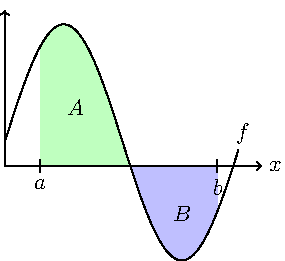
\includegraphics[scale=0.9]{../../asymptote/int6a}\quad
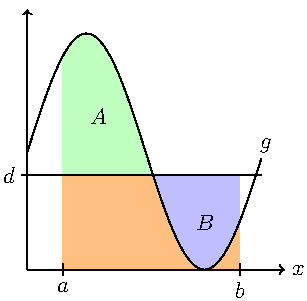
\includegraphics[scale=0.9]{../../asymptote/int6b}
\end{figure}
Forklar ut ifra en arealbetraktning hvorfor\[ \int\limits_a^b f \,dx=\int\limits_a^b g\,dx -(b-a)d  \]
\textbf{b)} Bekreft likheten i oppgave a) ved integrasjon.
\newpage
\opl{fogF}
Under vises grafen til $ F(x) $ og $ f(x) $. $ F $ er en antiderivert av $ f $.
\begin{figure}
	\centering
	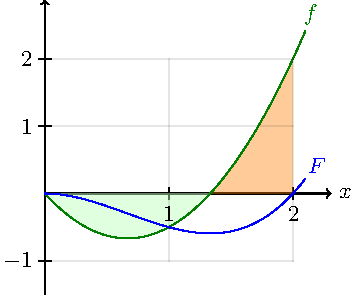
\includegraphics[scale=0.9]{../../asymptote/faropg}\\
	\raggedright
\end{figure}


Forklar hvorfor arealet av det oransje området er like stort som arealet av det grønne området.

\nes
\opl{kulevolopg}
La en kule med radius $ r $ være plassert i et koordinatsystem med variabelen $ x $ langs horisontalaksen. Kula er plassert slik at sentrum ligger i origo.\os

\textbf{a)} Lag en tegning og bestem kulas tverrsnitt $ A $ langs horisontalaksen, uttrykt ved $ r $ og $ x $.\os

\textbf{b)} Finn volumet $ V $ av kula.

\opl{omdropg} 
Finn volumet av omdreiningslegemene til funksjonene på intervallet $ [0, 1] $:\os

\begin{tabular}{@{}l l l}	
	\textbf{a)} $ f(x)=e^x  $&\quad\textbf{b)} $\displaystyle f(x)= \frac{1}{\sqrt{2}}\sqrt{1-\cos(2 \pi x)}$ &\quad
\end{tabular}

\ekspop
Bruk definisjonen fra (\ref{bint}) til å vise at
\[ \int\limits_a^b x^2 \,dx = \frac{1}{3}(b^3-a^3) \]
\textsl{Hint}: Bruk summen av de naturlige tallene og \eqref{sumkvad} fra s. \pageref{sumkvad}.



\begin{comment}
	\subsection*{GeoGebra-oppgaver}
	\op
	Hvis $ |x|\ll 1 $ kan man gjøre følgende tilnærming:
	\[f(x)= \frac{1}{\cos^2 {x}} \approx g(x)=1 + x^2 + \frac{2}{3}x^4 \]
	
	\textbf{a)} Tegn $ f(x) $ og $ g(x) $ inn i et koordinatsystem for $ x\in  [-0.4, 0.4]$
	
	\textbf{b)} Bruk det faktum at $  \int f(x)\, dx = \tan x $ og at $ \int f(x)\, dx \approx \int g(x)\, dx$ for å finne en tilnærming til $ \tan x $
\end{comment}
\end{document}